\section{Casi d'uso}
    \subsection{Attori dei casi d'uso}
    \subsubsection{Attori primari}
    Gli attori che il gruppo ha ritenuto essere i più adeguati sono:
        \begin{itemize}
            \item \textbf{Utente generico:} utente che può navigare nell'e-commerce e può usufruire di alcune funzionalità, come la visualizzazione e la ricerca dei prodotti, che può aggiungere al proprio carrello, la applicazione di filtri e categorie per la ricerca, e infine di potersi autenticare.\\ Inoltre si divide in:
                \begin{itemize}
                    \item \textbf{Utente non autenticato:} è un utente che ha già un account ma che non ha ancora effettuato il login; può quindi reimpostare la sua password nel caso in cui se la sia dimenticata;
                    \item \textbf{Utente autenticato:} un utente autenticato può a sua volta essere:
                        \begin{itemize}
                            \item \textbf{Cliente autenticato:} cliente che ha effettuato il login, può accedere a tutte le funzionalità riservate ai clienti, come l'aggiunta di prodotti al carrello, l'acquisto, la visualizzazione della lista degli ordini, la possibilità di contattare il venditore, la possibilità di effettuare un reso;
                            \item \textbf{Venditore autenticato:} venditore che ha effettuato il login, può accedere alle funzionalità relative all'amministrazione dei prodotti e delle categorie.
                        \end{itemize}
                        \begin{figure}[!ht]
                            \caption{Attori primari}
                            \vspace{5px}
                            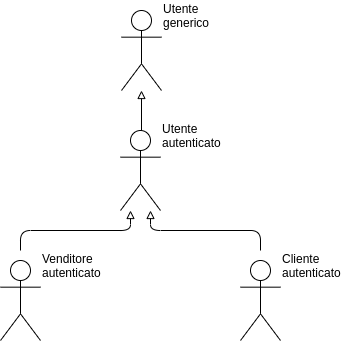
\includegraphics[scale=0.6]{../../../Images/AnalisiRequisiti/attori}
                            \centering
                        \end{figure}
                \end{itemize}
        \end{itemize}
        \subsubsection{Attori secondari}
        \begin{itemize}
            \item \textbf{Amazon Cognito:} servizio esterno per il login e per la gestione delle credenziali;
            \item \textbf{Stripe:} servizio esterno per la gestione dei pagamenti.
        \end{itemize}
        \newpage
    \subsection{Elenco dei casi d'uso}
        \textbf{Utilizzo della piattaforma:}
        \begin{figure}[!ht]
            \caption{Casi d'uso che interessano gli utenti}
            \vspace{10px}
            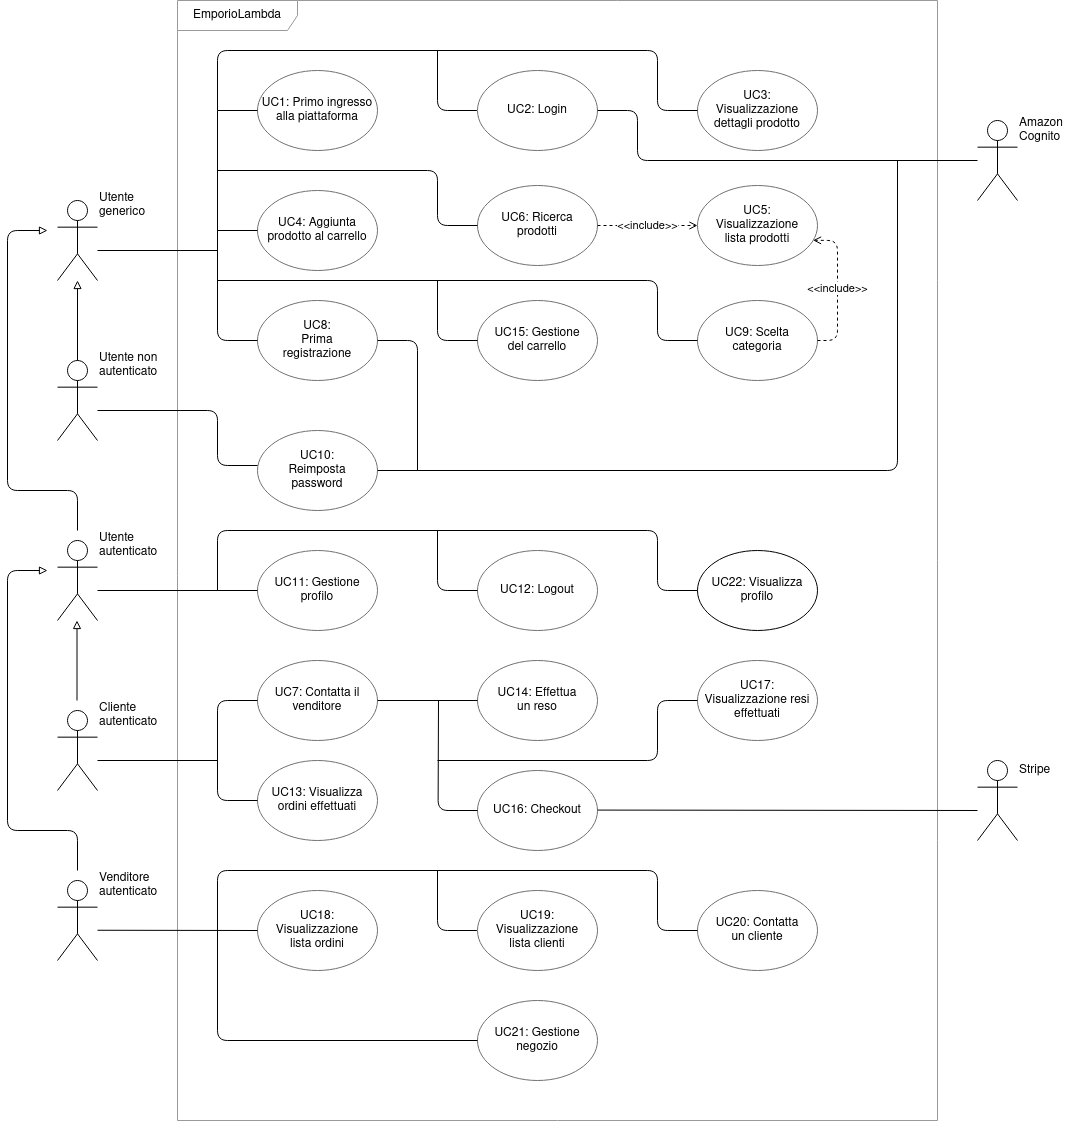
\includegraphics[scale=0.44]{../../../Images/AnalisiRequisiti/casiUso}
            \centering
        \end{figure}
        \newpage
        \subsection{UC1: Primo ingresso alla piattaforma}
        \label{sec:UC1}
        \begin{itemize}
            \item \textbf{Descrizione:} l'utente effettua il primo accesso alla piattaforma;
            \item \textbf{Attore Primario:} utente generico;
            \item \textbf{Precondizione:} l'utente non sta visualizzando nulla;
            \item \textbf{Postcondizione:} l'utente visualizza l'homepage della piattaforma;
            \item \textbf{Scenario Principale:} 
            \begin{itemize}
                \item l'utente arriva per la prima volta nell'e-commerce;
                \item visualizza l'homepage.
            \end{itemize}
        \end{itemize}
        \subsection{UC2: Login}
        \label{sec:UC2}
        \begin{itemize}
            \item \textbf{Descrizione:} permette l'autenticazione di un utente;
            \item \textbf{Attore Primario:} utente generico;
            \item \textbf{Attore Secondario:} Amazon Cognito;
            \item \textbf{Precondizione:} l'utente generico non si è ancora autenticato
            \item \textbf{Input:} pressione bottone login;
            \item \textbf{Postcondizione:} l'utente è autenticato;
            \item \textbf{Scenario Principale:} 
            \begin{itemize}
                \item l'utente entra nella pagina
                \item preme il bottone per il login
                \item viene inderizzato alla pagina di login fornita da \textit{Amazon Cognito}.
            \end{itemize}
        \end{itemize}
        \subsection{UC3: Visualizzazione dei dettagli di un prodotto}
        \label{sec:UC3}
        \begin{itemize}
            \item \textbf{Descrizione:} l'utente può visualizzare i dettagli di un prodotto di suo interesse;
            \item \textbf{Attore Primario:} utente generico
            \item \textbf{Precondizione:} l'utente generico si trova nella pagina della lista dei prodotti;
            \item \textbf{Input:} click sul prodotto (icona, immagine, nome);
            \item \textbf{Postcondizione:} l'utente visualizza i dettagli del prodotto d'interesse;
            \item \textbf{Scenario Principale:} 
                \begin{itemize}
                    \item l'utente si trova nella lista dei prodotti (\hyperref[sec:UC6]{\underline{UC6}});
                    \item l'utente visualizza un prodotto di suo interesse;
                    \item l'utente lo apre e ne visualizza i dettagli.
                \end{itemize}
        \end{itemize}
        \subsection{UC4: Aggiunta di un prodotto al carrello}
        \label{sec:UC4}
        \begin{itemize}
            \item \textbf{Descrizione:} l'utente aggiunge al carrello un prodotto che intende acquistare;
            \item \textbf{Attore Primario:} utente generico;
            \item \textbf{Precondizione:} l'utente generico di trova nella pagina dettagliata del prodotto (\hyperref[sec:UC3]{\underline{UC3}});
            \item \textbf{Input:} click sul bottone di aggiunta al carrello;
            \item \textbf{Postcondizione:} il prodotto è stato aggiunto al carrello;
            \item \textbf{Scenario Principale:}
            \begin{itemize}
                \item l'utente si trova nella pagina dei dettagli del prodotto;
                \item l'utente clicca il bottone per aggiungere il prodotto al carrello;
                \item il prodotto si trova nel carrello.
            \end{itemize}
        \end{itemize}
        \subsection{UC5: Ricerca dei prodotti}
        \label{sec:UC5}
        \begin{itemize}
            \item \textbf{Descrizione:} l'utente vuole ricercare un prodotto in base ad una parola chiave; 
            \item \textbf{Attore Primario:} utente generico;
            \item \textbf{Precondizione:} l'utente si trova in una pagina dedicata alla ricerca; 
            \item \textbf{Input:} stringa relativa a ciò che si vuole cercare;
            \item \textbf{Postcondizione:} l'utente visualizza i prodotti corrispondenti alla parola chiave;
            \item \textbf{Scenario Principale:}
            \begin{itemize}
                \item l'utente vuole ricercare un prodotto secondo una determinata parola chiave;
                \item gli vengo mostrati tutti i risultati della ricerca nella lista dei prodotti.
            \end{itemize}
            \item \textbf{Inclusioni:}
            \begin{itemize}
                \item viene visualizzata una pagina con tutti i risultati della ricerca \hyperref[sec:UC6]{\underline{UC6}}.
            \end{itemize}
        \end{itemize}
        \subsection{UC6: Visualizzazione della lista dei prodotti}
        \label{sec:UC6}
        \begin{figure}[!ht]
            \caption{Visualizzazione della lista dei prodotti}
            \vspace{10px}
            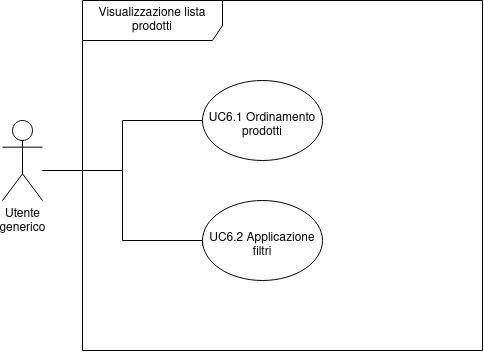
\includegraphics[scale=0.5]{../../../Images/AnalisiRequisiti/UC6.png}
            \centering
        \end{figure}
        \begin{itemize}
            \item \textbf{Descrizione:} l'utente visualizza la pagina della lista dei prodotti;
            \item \textbf{Attore Primario:} utente generico;
            \item \textbf{Precondizione:} l'utente si trova in una qualsiasi pagina della piattaforma;
            \item \textbf{Postcondizione:} l'utente visualizza la pagina con la lista dei prodotti;
            \item \textbf{Scenario Principale:}
            \begin{itemize}
                \item l'utente è in una pagina della piattaforma;
                \item cerca un prodotto o sceglie una categoria;
                \item l'utente visualizza la lista dei prodott.
            \end{itemize}
        \end{itemize}
        \subsubsection{UC6.1: Ordinamento prodotti}
        \label{sec:UC6.1}
        \begin{itemize}
            \item \textbf{Descrizione:} l'utente seleziona la modalità in cui visualizzare i file;
            \item \textbf{Attore Primario:} utente generico;
            \item \textbf{Precondizione:} l'utente si trova all'interno della pagina con la lista dei prodotti;
            \item \textbf{Input:} selezione del parametro scelto;
            \item \textbf{Postcondizione:} la lista dei prodotti si aggiorna secondo l'ordinamento scelto;
            \item \textbf{Scenario Principale:}
            \begin{itemize}
                \item l'utente si trova all'interno della pagina con la lista dei prodotti;
                \item inserisce i parametri per ordinare i prodotti;
                \item la pagina con la lista dei prodotti si aggiorna con i prodotti ordinati.
            \end{itemize}
        \end{itemize}
        \subsubsection{UC6.2: Applicazione filtri}
        \label{sec:UC6.2}
        \begin{itemize}
            \item \textbf{Descrizione:} l'utente filtra i prodotti in base alle loro caratteristiche;
            \item \textbf{Attore Primarilo:} utente generico
            \item \textbf{Precondizione:} l'utente si trova all'interno della pagina con la lista dei prodotti;
            \item \textbf{Input:} selezione del filtro desiderato;
            \item \textbf{Postcondizione:} la pagina si aggiorna secondo i filtri selezionati;
            \item \textbf{Scenario Principale:}
            \begin{itemize}
                \item l'utente si trova all'interno della pagina con la lista dei prodotti;
                \item inserisce i parametri per filtrare i prodotti;
                \item la pagina con la lista dei prodotti si aggiorna con i prodotti filtrati.
            \end{itemize}
        \end{itemize}
        \subsection{UC7: Contatta il venditore}
        \label{sec:UC7}
        \begin{itemize}
            \item \textbf{Descrizione:} l'utente vuole contattare il venditore;
            \item \textbf{Attore Primario:} utente autenticato
            \item \textbf{Precondizione:} l'utente si trova in una pagina che permette di contattare il venditore;
            \item \textbf{Input:} pressione dell'apposito bottone;
            \item \textbf{Postcondizione:} l'utente può contattare il venditore;
            \item \textbf{Scenario Principale:}
            \begin{itemize}
                \item l'utente contatta il venditore tramite questa sezione.
            \end{itemize}
        \end{itemize}
        \subsection{UC8: Prima registrazione}
        \label{sec:UC8}
        \begin{itemize}
            \item \textbf{Descrizione:} l'utente non si è mai registrato nella piattaforma;
            \item \textbf{Attore Primario:} utente generico;
            \item \textbf{Attore Secondario:} Amazon Cognito;
            \item \textbf{Precondizione:} l'utente non ha un profilo nella piattaforma;
            \item \textbf{Input:} pressione apposito bottone;
            \item \textbf{Postcondizione:} l'utente viene reinderizzato alla pagina Amazon cognito per la registrazione;
            \item \textbf{Scenario Principale:}
            \begin{itemize}
                \item un utente arriva per la prima volta nella piattaforma;
                \item si registra attraverso la piattaforma Amazon Cognito dove potrà registrarsi inserendo:
                \begin{itemize}
                    \item nome;
                    \item cognome;
                    \item username;
                    \item password;
                    \item ripetizione password.
                \end{itemize}
            \end{itemize} 
        \end{itemize}
        \subsection{UC9: Scelta della categoria}
        \label{sec:UC9}
        \begin{itemize}
            \item \textbf{Descrizione:} l'utente sceglie una specifica categoria di prodotti da ricercare;
            \item \textbf{Attore Primario:} utente generico;
            \item \textbf{Precondizione:} l'utente si trova in una pagina che consente la divisione in categorie;
            \item \textbf{Input:} selezione della categoria;
            \item \textbf{Postcondizione:} la categoria di ricerca cambia secondo la scelta dell'utente;
            \item \textbf{Scenario Principale:}
            \begin{itemize}
                \item l'utente vuole ricercare un prodotto appartenente ad una determinata categoria.
            \end{itemize} 
            \item \textbf{Inclusioni:}
            \begin{itemize}
                \item viene visualizzata una pagina con tutti i risultati della ricerca \hyperref[sec:UC6]{\underline{UC6}}.
            \end{itemize}
        \end{itemize}
        \subsection{UC10: Reimposta password (dimenticata)}
        \label{sec:UC10}
        \begin{itemize}
            \item \textbf{Descrizione:} l'utente non ricorda le prorpie credenziali;
            \item \textbf{Attore Primario:} Amazon Cognito;
            \item \textbf{Precondizione:} l'utente si trova nella pagina di login;
            \item \textbf{Input:} pressione apposito bottone;
            \item \textbf{Postcondizione:} l'utente viene reindirizzato alla pagina di recupero password;
            \item \textbf{Scenario Principale:}
            \begin{itemize}
                \item un utente non ancora autenticato, non ricorda la proprio password;
                \item procede con la procedura di recupero.
            \end{itemize}
        \end{itemize}
        \subsection{UC11: Gestione profilo}
        \label{sec:UC11}
        \begin{itemize}
            \item \textbf{Descrizione:} l'utente vuole gestire il proprio profilo;
            \item \textbf{Attore Primario:} utente autenticato;
            \item \textbf{Attore Secondario:} Amazon Cognito;
            \item \textbf{Precondizione:} l'utente si trova all'interno del suo profilo
            \item \textbf{Postcondizione:} l'utente può modificare il proprio profilo
            \item \textbf{Scenario Principale:}
            \begin{itemize}
                \item  l'utente può modificare:
                \begin{itemize}
                    \item nome;
                    \item cognome;
                    \item username;
                    \item password
                    \item indirizzi.
                \end{itemize}
            \end{itemize}
        \end{itemize}

        
        \subsection{UC12: Logout}
        \begin{itemize}
            \item \textbf{Descrizione:} sezione per effettuare il logout;
            \item \textbf{Attore Primario:} utente autenticato;
            \item \textbf{Precondizione:} l'utente (cliente o venditore) si trova in una qualsiasi pagina della piattaforma;
            \item \textbf{Input:} l'utente clicca il bottone apposito per effettuare il logout;
            \item \textbf{Postcondizione:} l'utente diventa non autenticato, uscendo dalla sessione.
            \item \textbf{Scenario Principale:}
            \begin{itemize}
                \item l'utente autenticato preme il pulsante per terminare la sessione ed effettua il logout.
            \end{itemize}
        \end{itemize}


        \subsection{UC13: Visualizza gli ordini effettuati}
        \label{sec:UC13}
        \begin{itemize}
            \item \textbf{Descrizione:} sezione per visualizzare l'elenco degli ordini effettuati;
            \item \textbf{Attore Primario:} cliente autenticato;
            \item \textbf{Precondizione:} il cliente si trova in una qualsiasi pagina della piattaforma;
            \item \textbf{Input:} il cliente clicca il bottone apposito per entrare il questa sezione;
            \item \textbf{Postcondizione:} il cliente visualizza l'elenco degli ordini che ha effettuato.
            \item \textbf{Scenario Principale:}
            \begin{itemize}
                \item l'utente si trova in una qualsiasi pagina;
                \item clicca il pulsante per visualizzare gli ordini e li visualizza.
            \end{itemize}
        \end{itemize}


        \subsection{UC14: Effettua un reso}
        \begin{itemize}
            \item \textbf{Descrizione:} sezione per effettuare il reso di un ordine;
            \item \textbf{Attore Primario:} cliente autenticato;
            \item \textbf{Precondizione:} il cliente si trova nella pagina per la visualizzazione dell'elenco degli ordini (\hyperref[sec:UC13]{\underline{UC13}});
            \item \textbf{Input:} il cliente clicca il bottone per entrare in questa sezione;
            \item \textbf{Postcondizione:} la richiesta di reso è andata a buon fine e i prodotti dell'ordine torneranno al venditore;
            \item \textbf{Scenario Principale:}
                \begin{itemize}
                    \item il cliente si trova nella sezione per visualizzare gli ordini effettuati;
                    \item clicca il bottone per eseguire il reso di un ordine;
                    \item il cliente conferma e il reso è confermato.
                \end{itemize}
        \end{itemize}


        \subsection{UC15: Gestione del carrello}
        \begin{figure}[!ht]
            \caption{Diagramma di UC15: Gestione del carrello}
            \vspace{10px}
            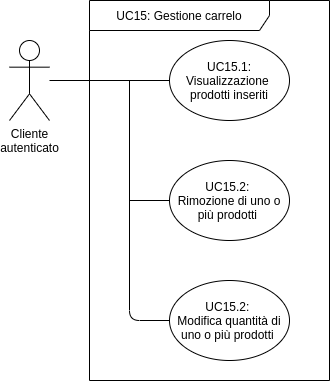
\includegraphics[scale=0.5]{../../../Images/AnalisiRequisiti/UC15}
            \centering
        \end{figure}
        \begin{itemize}
            \item \textbf{Descrizione:} questa sezione tratta l'insieme di operazioni che un utente generico fa per gestire i prodotti nel carrello;
            \item \textbf{Attore Primario:} utente generico;
            \item \textbf{Precondizione:} l'utente si trova in una qualsiasi pagina della piattaforma;
            \item \textbf{Input:} l'utente clicca il bottone per entrare nel carrello;
            \item \textbf{Postcondizione:} l'utente ha completato le operazioni per gestire i prodotti nel carrello;
            \item \textbf{Scenario Principale:}
                \begin{itemize}
                    \item l'utente si trova in una qualsiasi pagina della piattaforma;
                    \item clicca il bottone per entrare nel carrello;
                    \item una volta entrato vede la lista di tutti i prodotti all'interno del carrello;
                    \item può decidere se rimuovere qualche prodotto o modificarne le quantità.
                \end{itemize}
        \end{itemize}
        \subsubsection{UC15.1: Visualizzazione dei prodotti inseriti}
        \label{sec:UC15.1}
        \begin{itemize}
            \item \textbf{Descrizione:} sezione per visualizzare tutti i prodotti inseriti nel carrello;
            \item \textbf{Attore Primario:} utente generico;
            \item \textbf{Precondizione:}  l'utente si trova in una qualsiasi pagina della piattaforma;
            \item \textbf{Input:} l'utente clicca il bottone per entrare nel carrello;
            \item \textbf{Postcondizione:} l'utente si trova sulla pagina del carrello e vede tutti i prodotti presenti al suo interno;
            \item \textbf{Scenario Principale:}
                \begin{itemize}
                    \item l'utente si trova in una pagina della piattaforma;
                    \item l'utente clicca il bottone per entrare nel carrello;
                    \item una volta entrato l'elenco dei prodotti è subito visibile.
                \end{itemize}
        \end{itemize}
        \subsubsection{UC15.2: Rimozione di uno o più prodotti}
        \begin{itemize}
            \item \textbf{Descrizione:} sezione per rimuovere uno o più prodotti dal carrello;
            \item \textbf{Attore Primario:} utente generico;
            \item \textbf{Precondizione:} l'utente è nella pagina del carrello (\hyperref[sec:UC15.1]{\underline{UC15.1}});
            \item \textbf{Input:} l'utente seleziona i prodotti da rimuovere dal carrello;
            \item \textbf{Postcondizione:} vengono rimossi i prodotti selezionati;
        \end{itemize}
        \subsubsection{UC15.3: Modifica della quantità di uno o più prodotti}
        \begin{itemize}
            \item \textbf{Descrizione:} sezione per modificare le quantità dei prodotti nel carrello;
            \item \textbf{Attore Primario:} utente generico;
            \item \textbf{Precondizione:} l'utente è nella pagina del carrello (\hyperref[sec:UC15.1]{\underline{UC15.1}});
            \item \textbf{Input:} l'utente inserisce le modifiche desiderate ai prodotti;
            \item \textbf{Postcondizione:} le modifiche sono applicate;
            \item \textbf{Estensioni:} 
                \begin{itemize}
                    \item se la nuova quantità non dovesse essere disponibile per il venditore, l'utente viene avvisato.
                \end{itemize}
        \end{itemize}

        
        \subsection{UC16: Checkout}
            \begin{figure}[!ht]
                \caption{Diagramma di UC16: Checkout}
                \vspace{10px}
                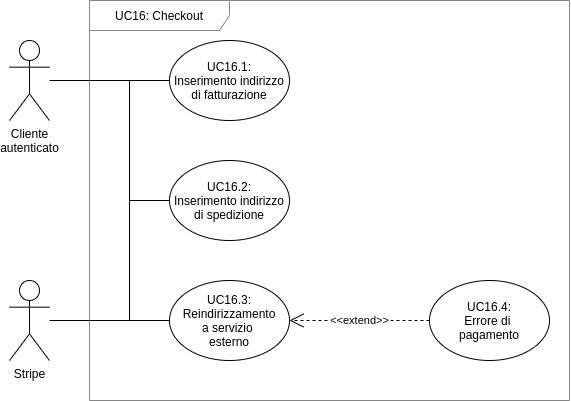
\includegraphics[scale=0.5]{../../../Images/AnalisiRequisiti/UC16}
                \centering
            \end{figure}
                \begin{itemize}
                \item \textbf{Descrizione:} caso d'uso per la creazione di un nuovo ordine e l'acquisto dei prodotti inseriti nel carrello;
                \item \textbf{Attore Primario:} cliente autenticato;
                \item \textbf{Attore Secondario:} Stripe, gestore di pagamenti di terze parti;
                \item \textbf{Precondizione:} il cliente si trova sul carrello e ha già inserito almeno un prodotto;
                \item \textbf{Input:} il cliente clicca il bottone per iniziare il checkout;
                \item \textbf{Postcondizione:} l'ordine viene emesso e aggiunto alla lista degli ordini di quel cliente; i prodotti acquistati vengono rimossi dal carrello e viene diminuita la quantità dal deposito del venditore;
                \item \textbf{Scenario Principale:} 
                    \begin{itemize}
                        \item il cliente preme sul pulsante per entrare nella sezione del checkout;
                        \item il cliente inserisce i dati di fatturazione (\hyperref[sec:UC16.1]{\underline{UC16.1}}) e, se diversi, i dati di spedizione (\hyperref[sec:UC16.2]{\underline{UC16.2}});
                        \item vengono inseriti eventuali costi di spedizione;
                        \item il cliente viene reindirizzato al servizio di pagamento esterno, dove inserisce i dati di pagamento;
                        \item l'ordine è emesso e segnato come completato.
                    \end{itemize}
                \item \textbf{Estensioni:}
                    \begin{itemize}
                        \item se il cliente decide di non completare il checkout, può uscire dalla pagina senza causare modifiche al carrello;
                        \item se il pagamento ha avuto esito negativo, l'ordine non viene emesso e quindi è necessario ricominciare il pagamento.
                    \end{itemize}
            \end{itemize}
            \subsubsection{UC16.1: Inserimento dell'indirizzo di fatturazione}
            \label{sec:UC16.1}
                \begin{itemize}
                    \item \textbf{Descrizione:} Sezione per l'inserimento dell'indirizzo fatturazione;
                    \item \textbf{Attore Primario:} cliente autenticato;
                    \item \textbf{Precondizione:} il cliente si trova nella fase di checkout;
                    \item \textbf{Input:} il cliente inserisce i dati richiesti dalla pagina;
                    \item \textbf{Postcondizione:} si procede con la fase successiva del checkout (\hyperref[sec:UC16.2]{\underline{UC16.2}})
                    \item \textbf{Scenario Principale:} il cliente inserisce negli appositi spazi i dati per completare l'indirizzo di fatturazione.
                \end{itemize}
            \subsubsection{UC16.2: Inserimento dell'indirizzo di spedizione}
            \label{sec:UC16.2}
                \begin{itemize}
                    \item \textbf{Descrizione:} Sezione per l'inserimento dell'indirizzo spedizione;
                    \item \textbf{Attore Primario:} cliente autenticato;
                    \item \textbf{Precondizione:} il cliente si trova nella fase di checkout;
                    \item \textbf{Input:} il cliente inserisce i dati richiesti dalla pagina, oppure clicca un pulsante se l'indirizzo di spedizione è lo stesso di quello di fatturazione;
                    \item \textbf{Postcondizione:} si procede con la fase successiva del checkout (\hyperref[sec:UC16.3]{\underline{UC16.3}})
                    \item \textbf{Scenario Principale:} il cliente inserisce negli appositi spazi i dati per completare l'indirizzo di spedizione oppure clicca il pulsante per autocompletarli se è il medesimo di quello di fatturazione.
                \end{itemize}
            \subsubsection{UC16.3: Reindirizzamento al servizio di pagamento esterno}
            \label{sec:UC16.3}
                \begin{itemize}
                    \item \textbf{Descrizione:} Sezione per il pagamento dell'ordine da effettuare;
                    \item \textbf{Attore Primario:} cliente autenticato;
                    \item \textbf{Attore Secondario:} Stripe, gestore di pagamenti di terze parti;
                    \item \textbf{Precondizione:} il cliente ha inserito i dati per la fatturazione e la spedizione nella sezione del checkout;
                    \item \textbf{Input:} il cliente preme il pulsante per il pagamento;
                    \item \textbf{Postcondizione:} il pagamento ha avuto esito positivo, l'ordine viene confermato e viene decrementata la quantità dei prodotti disponibili al venditore, in base al numero di prodotti acquistati dal cliente;
                    \item \textbf{Scenario Principale:}
                    \begin{itemize}
                        \item il cliente preme sul pulsante e viene reindirizzato al servizio esterno per eseguire il pagamento;
                        \item il cliente inserisce i propri dati ed esegue il pagamento;
                        \item il pagamento è riuscito e l'ordine viene confermato.
                    \end{itemize}
                    \item \textbf{Estensioni:}
                    \begin{itemize}
                        \item il pagamento non è riuscito, viene visualizzato un errore di pagamento (\hyperref[sec:UC16.4]{\underline{UC16.4}}) e si viene reindirizzati alla pagina del checkout per riprovare.
                    \end{itemize}
                \end{itemize}
            \subsubsection{UC16.4: Errore di pagamento}
            \label{sec:UC16.4}
                \begin{itemize}
                    \item \textbf{Descrizione:} visualizzazione di un errore per un fallimento nella fase di pagamento;
                    \item \textbf{Attore Primario:} Stripe
                    \item \textbf{Precondizione:} il cliente ha inserito i dati del pagamento;
                    \item \textbf{Input:} Stripe ritorna un errore nel risultato del pagamento;
                    \item \textbf{Postcondizione:} viene visualizzato un messaggio di errore, successivamente il cliente viene reindirizzato alla sezione del checkout;
                \end{itemize}


        \subsection{UC17: Visualizzazione dei resi effettuati}
            \begin{itemize}
                \item \textbf{Descrizione:} sezione per visualizzare l'elenco dei resi effettuati;
                \item \textbf{Attore Primario:} cliente autenticato;
                \item \textbf{Precondizione:} l'utente si trova nella sezione degli ordini effettuati (\hyperref[sec:UC18]{\underline{UC18}})
                \item \textbf{Input:} l'utente clicca il bottone apposito per entrare il questa sezione;
                \item \textbf{Postcondizione:} l'utente visualizza l'elenco dei resi che ha effettuato;
            \end{itemize}


        \subsection{UC18: Visualizzazione della lista degli ordini}
        \label{sec:UC18}
        \begin{itemize}
            \item \textbf{Descrizione:} sezione per visualizzare l'elenco degli ordini effettuati dai clienti;
            \item \textbf{Attore Primario:} venditore autenticato; 
            \item \textbf{Precondizione:} il venditore si trova in una qualsiasi pagina della piattaforma;
            \item \textbf{Input:} il venditore clicca il bottone per entrare in questa sezione; 
            \item \textbf{Postcondizione:} il venditore visualizza la lista di tutti gli ordini effettuati dai suoi clienti.
        \end{itemize}


        \subsection{UC19: Visualizzazione della lista dei clienti}
        \label{sec:UC19}
            \begin{itemize}
                \item \textbf{Descrizione:} sezione per visualizzare l'elenco dei clienti del proprio negozio;
                \item \textbf{Attore Primario:} venditore autenticato; 
                \item \textbf{Precondizione:} il venditore si trova in una qualsiasi pagina;
                \item \textbf{Input:} il venditore clicca il bottone per entrare in questa sezione; 
                \item \textbf{Postcondizione:} il venditore visualizza la lista di tutti i clienti del negozio.
                \end{itemize}


        \subsection{UC20: Contatta un cliente}
        \begin{itemize}
            \item \textbf{Descrizione:} sezione per il venditore che permette di contattare un cliente;
            \item \textbf{Attore Primario:} venditore autenticato;
            \item \textbf{Precondizione:} il venditore si trova nella lista dei suoi clienti (\hyperref[sec:UC19]{\underline{UC19}});
            \item \textbf{Input} il venditore clicca il bottone per entrare in questa sezione; 
            \item \textbf{Postcondizione:} il venditore ha inviato una e-mail ad un suo cliente;
            \item \textbf{Scenario Principale}
                \begin{itemize}
                    \item il venditore si trova nella lista dei suoi clienti;
                    \item sceglie uno dei suoi clienti per poterlo contattare;
                    \item compila il campo di testo scrivendo ciò che deve inviare;
                    \item preme il pulsante per inviare, una e-mail verrà inviata al cliente;
                \end{itemize}
        \end{itemize}

        \subsection{UC21: Gestione del negozio }
        \label{sec:UC21}
        \begin{itemize}
            \begin{figure}
                \caption{Diagramma di UC21: Gestione del negozio}
                \vspace{10px}
                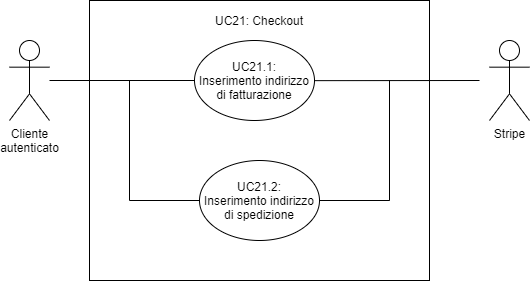
\includegraphics[scale=0.5]{../../../Images/AnalisiRequisiti/UC21}
                \centering
            \end{figure}
            \item \textbf{Descrizione:} sezione per il venditore, dove può gestire le parti relative al negozio;
            \item \textbf{Attore Primario:} venditore autenticato;
            \item \textbf{Precondizione:} il venditore si trova in una qualsiasi pagina;
            \item \textbf{Input:} il venditore preme il bottone per entrare in questa sezione;
            \item \textbf{Postcondizione:} il venditore ha completato le modifiche desiderate;
            \item \textbf{Scenario Principale:} 
                \begin{itemize}
                    \item il venditore si trova in una pagina della piattaforma e preme il bottone per entrare in questa sezione;
                    \item può gestire i prodotti presenti nel negozio;
                    \item può gestire le categorie per permettere ai clienti di individuare meglio i prodotti;
                    \item una volta terminato applica le modifiche.
                \end{itemize}
        \end{itemize}
        \subsubsection{UC21.1: Gestione dei prodotti}
        \label{sec:UC21.1}
        \begin{figure}[!ht]
            \caption{Diagramma di UC21.1: Gestione dei prodotti}
            \vspace{10px}
            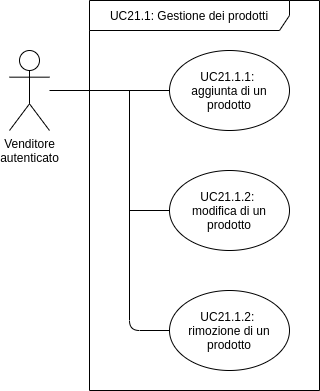
\includegraphics[scale=0.5]{../../../Images/AnalisiRequisiti/UC21.1}
            \centering
        \end{figure}
        \begin{itemize}
            \item \textbf{Descrizione:} sezione per il venditore, dove può gestire i prodotti del negozio;
            \item \textbf{Attore Primario:} venditore autenticato;
            \item \textbf{Precondizione:} il venditore si trova nella pagina per la gestione del negozio (\hyperref[sec:UC21]{\underline{UC21}});
            \item \textbf{Input:} il venditore preme il bottone per entrare in questa sezione;
            \item \textbf{Postcondizione:} il venditore ha completato le modifiche ai prodotti desiderati;
            \item \textbf{Scenario Principale:} 
                \begin{itemize}
                    \item il venditore si trova nella pagina per la gestione del negozio;
                    \item può decidere se aggiungere un nuovo prodotto, modificarne o rimuoverne uno già presente;
                    \item una volta terminato applica le modifiche
                \end{itemize}
        \end{itemize}
        \subsubsubsection{UC21.1.1: Aggiunta di un prodotto}
        \begin{itemize}
            \item \textbf{Descrizione:} sezione per aggiungere un prodotto nel negozio;
            \item \textbf{Attore Primario:} venditore autenticato;
            \item \textbf{Precondizione:} il venditore si trova nella sezione per gestire i prodotti (\hyperref[sec:UC21.1]{\underline{UC21.1}});
            \item \textbf{Input:} il venditore inserisce tutti i dati relativi al prodotto da inserire;
            \item \textbf{Postcondizione:} il prodotto è aggiunto e i clienti possono trovarlo nel negozio;
            \item \textbf{Scenario Principale:} 
                \begin{itemize}
                    \item il venditore si trova nella sezione per gestire i prodotti;
                    \item il venditore decide di aggiungere un nuovo prodotto ed entra in questa sezione;
                    \item inserisce tutti i dati richiesti (nome, descrizione, prezzo ecc.);
                    \item conferma l'aggiunta e il prodotto è disponibile nel negozio.
                \end{itemize}
        \end{itemize}
        \subsubsubsection{UC21.1.2: Modifica di un prodotto}
        \begin{itemize}
            \item \textbf{Descrizione:} sezione per modificare un prodotto del negozio;
            \item \textbf{Attore Primario:} venditore autenticato;
            \item \textbf{Precondizione:} il venditore si trova nella sezione per gestire i prodotti (\hyperref[sec:UC21.1]{\underline{UC21.1}});
            \item \textbf{Input:} il venditore modifica i dati che ritiene opportuni relativi al prodotto da modificare;
            \item \textbf{Postcondizione:} il prodotto è stato modificato;
            \item \textbf{Scenario Principale:} 
                \begin{itemize}
                    \item il venditore si trova nella sezione per gestire i prodotti;
                    \item il venditore decide di modificare un prodotto ed entra in questa sezione;
                    \item modifica i dati che preferisce;
                    \item conferma le modifiche.
                \end{itemize}
        \end{itemize}
        \subsubsubsection{UC21.1.3: Rimozione di un prodotto}
        \begin{itemize}
            \item \textbf{Descrizione:} sezione per rimuovere un prodotto dal negozio;
            \item \textbf{Attore Primario:} venditore autenticato;
            \item \textbf{Precondizione:} il venditore si trova nella sezione per gestire i prodotti (\hyperref[sec:UC21.1]{\underline{UC21.1}});
            \item \textbf{Input:} il venditore sceglie il prodotto da eliminare;
            \item \textbf{Postcondizione:} il prodotto è stato rimosso dal negozio;
            \item \textbf{Scenario Principale:} 
                \begin{itemize}
                    \item il venditore si trova nella sezione per gestire i prodotti;
                    \item il venditore decide di rimuovere un prodotto dal negozio;
                    \item conferma;
                    \item il prodotto non è più visibile nel negozio.
                \end{itemize}
        \end{itemize}


        \subsubsection{UC21.2: Gestione delle categorie}
        \label{sec:UC21.2}
        \begin{figure}[!ht]
            \caption{Diagramma di UC21.2: Gestione delle categorie}
            \vspace{10px}
            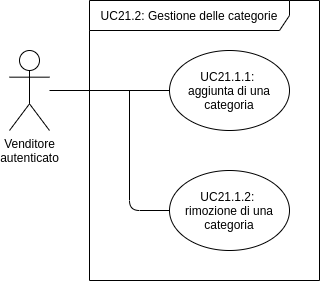
\includegraphics[scale=0.5]{../../../Images/AnalisiRequisiti/UC21.2}
            \centering
        \end{figure}
        \begin{itemize}
            \item \textbf{Descrizione:} sezione per il venditore, dove può gestire le categorie del negozio;
            \item \textbf{Attore Primario:} venditore autenticato;
            \item \textbf{Precondizione:} il venditore si trova nella pagina per la gestione del negozio (\hyperref[sec:UC21]{\underline{UC21}});
            \item \textbf{Input:} il venditore preme il bottone per entrare in questa sezione;
            \item \textbf{Postcondizione:} il venditore ha completato le operazioni sulle categorie;
            \item \textbf{Scenario Principale:} 
                \begin{itemize}
                    \item il venditore si trova nella pagina per la gestione del negozio;
                    \item può decidere se aggiungere una nuova categoria o se rimuoverne una già presente;
                    \item una volta terminato applica le modifiche.
                \end{itemize}
        \end{itemize}
        \subsubsubsection{UC21.2.1: Aggiunta di una categoria}
        \begin{itemize}
            \item \textbf{Descrizione:} sezione per aggiungere una categoria di prodotti nel negozio;
            \item \textbf{Attore Primario:} venditore autenticato;
            \item \textbf{Precondizione:} il venditore si trova nella sezione per gestire le categorie (\hyperref[sec:UC21.2]{\underline{UC21.2}});
            \item \textbf{Input:} il venditore inserisce tutti i dati relativi alla categoria da inserire;
            \item \textbf{Postcondizione:} la categoria è aggiunta e i clienti possono trovarlo nel negozio;
            \item \textbf{Scenario Principale:} 
                \begin{itemize}
                    \item il venditore si trova nella sezione per gestire le categorie;
                    \item il venditore decide di aggiungere una nuova categoria ed entra in questa sezione;
                    \item inserisce tutti i dati richiesti;
                    \item conferma l'aggiunta e la categoria è visibile nel negozio.
                \end{itemize}
        \end{itemize}
        \subsubsubsection{UC21.2.2: Rimozione di una categoria}
        \begin{itemize}
            \item \textbf{Descrizione:} sezione per rimuovere una categoria dal negozio;
            \item \textbf{Attore Primario:} venditore autenticato;
            \item \textbf{Precondizione:} il venditore si trova nella sezione per gestire le categorie (\hyperref[sec:UC21.2]{\underline{UC21.2}});
            \item \textbf{Input:} il venditore sceglie la categoria da eliminare;
            \item \textbf{Postcondizione:} la categoria è stata rimossa dal negozio;
            \item \textbf{Scenario Principale:} 
                \begin{itemize}
                    \item il venditore si trova nella sezione per gestire le categorie;
                    \item il venditore decide di rimuovere una categoria dal negozio;
                    \item conferma;
                    \item la categoria non è più visibile nel negozio.
                \end{itemize}
        \end{itemize}
        \subsection{UC22: Visualizzazione profilo}
        \label{sec:UC22}
        \begin{itemize}
            \item \textbf{Descrizione:} l'utente vuole visualizzare le informazioni del proprio profilo;
            \item \textbf{Attore Primario:} Utente autenticato;
            \item \textbf{Attore Secondario:} Amazon Cognito;
            \item \textbf{Precondizione:} l'utente di trova all'interno della piattaforma;
            \item \textbf{Input:} pressione dell'apposito bottone;
            \item \textbf{Postcondizione:} L'utente viene reindirizzato alla pagnia del suo profilo.
            \item \textbf{Scenario Principale:} L'utente entra nel proprio profilo e vede le sue informazioni:
            \begin{itemize}
                \item nome;
                \item e-mail;
                \item indirizzi.
            \end{itemize}
        \end{itemize}

